\chapter{WLAN technologies and security}
With WLAN, as previously mentioned, we refer to a network that covers a small area. Actually, the most
common WLAN technology is Wi-Fi, which is based on IEEE 802.11 and trademarked.\\
Wifi supports mainly the infrastructure-based mode: which is usually made up of 
\begin{itemize}
  \item Access Points(APs)
  \item Wireless stations(STAs)
\end{itemize}
All the STAs are connected to the APs, which are connected to the wired network.\\
It actually supports ad-hoc mode, which uses direct communication, but it is not used that much.\\
  In infrastructure-based mode, all traffic must go through the AP, having no direct communication 
  possible. This is to solve the hidden terminal problem, where two STAs can't communicate because they
  can't hear each other, and 
\begin{figure}[h]
  \centering
  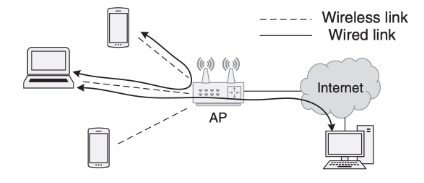
\includegraphics[width=0.7\textwidth]{img/wireless/wlan communication.png}
  \caption{Schema of a possible wireless communication}
\end{figure}
Furthermore, because it is based on 802.11, it carries over most of the standard:
\begin{itemize}
  \item \textbf{half-duplex communication channel}, at any time only one station can transmit or receive
  \item works on 2.4GHz and 5GHz bands, so multiplexing is available but quite limited
  \item uses \textbf{CSMA/CA} for medium access(carrier sense multiple access with collision avoidance)
\end{itemize}
The spectrum of the 2.4GHz band is divided into 14 channels, but only 3 of them are non-overlapping.
The 5GHz band has more channels, but it is less used because of the shorter range.
\begin{figure}
  \centering
  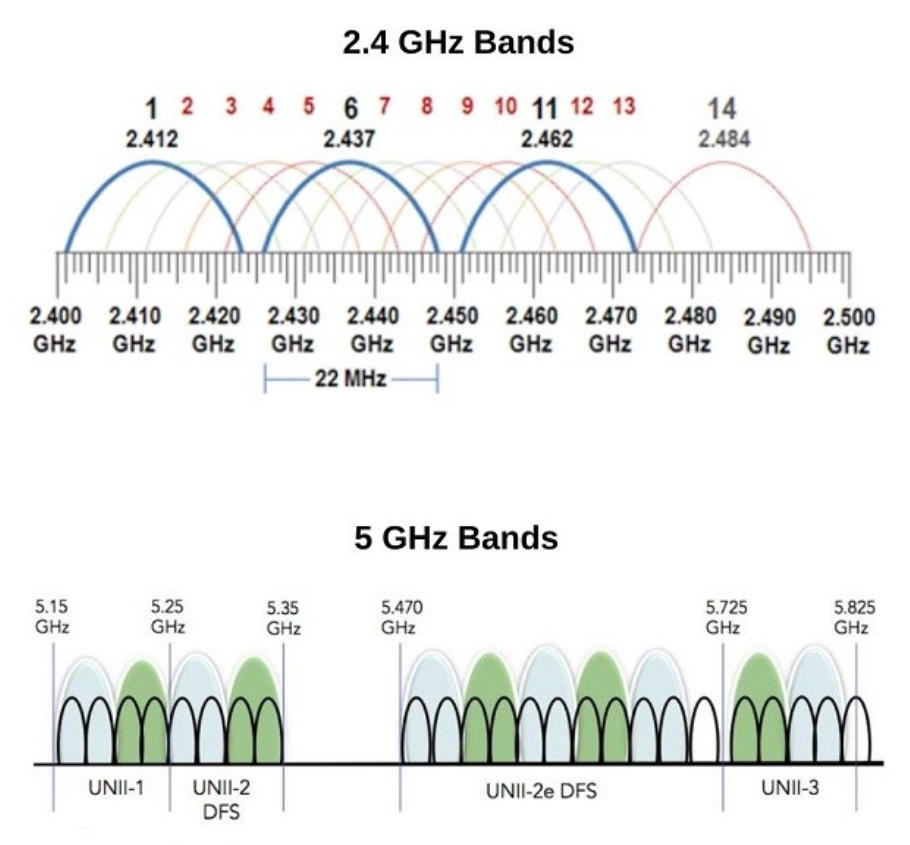
\includegraphics[width=0.5\textwidth]{img/wireless/80211 channels.png}
  \caption{802.11 channels}
\end{figure}
\begin{section}{WLAN Access}
  Before being able to access the network, an be able to send traffic trough an AP, a 
  mobile station can be:
  \begin{itemize}
    \item \textbf{Unauthenticated and unassociated}: the STA is not authenticated and not associated
    \item \textbf{Authenticated and unassociated}: the STA is authenticated but cannot transmit of receive 
      data
    \item \textbf{Authenticated and associated}: the STA is authenticated and associated
  \end{itemize}
  Data exchange is only possible in the last case.
  \begin{paragraph}{Authentication}
    The 802.11 authentication is the first step to be performed. It requires the STA to prove its identity
    to the AP. During this step, no data encryption or security in general is provided.\\
    Usually the authentication is done with a shared key(WEP, WPA, WPA2, WP3), but it can also be 
    done with open system authentication, where the AP accepts any STA that wants to connect.\\
  \end{paragraph}
  \begin{paragraph}{Association}
    The 802.11 association is the second step to be performed. It requires the STA to select the AP to connect to,
    and to exchange information with it to gain access to the network.\\
    Association allows the AP to record each STA so that frames can be sent to the correct destination.
    Association only works in infrastructure mode, and a station can only be associated with one AP at a time.
    It is usually carried out as follows:
    \begin{itemize}
      \item After authentication, the STA sends an association request to the AP
      \item The AP processes the Association Request and decides if a client request should be allowed
        \subitem If the request is accepted it responds with a status code of 0 (successful) and the 
        Association ID (AID)
        \subitem Failed Association Requests include only a status code and the procedure ends
    \end{itemize}
  \end{paragraph}
  The STA must go through the following steps:
  \begin{enumerate}
    \item \textbf{Scanning(Beacon/probe)}: the STA scans the environment to find the APs
    \item \textbf{Association}: the STA selects the AP and sends an association request
    \item \textbf{Authentication}: the AP sends an authentication request to the STA
    \item \textbf{Authentication}: the STA sends an authentication response to the AP
    \item \textbf{Association}: the AP sends an association response to the STA
    \item \textbf{Exchange of data}: the STA can now exchange data with the AP
  \end{enumerate}
  Authentication can be performed with multiple access points of the same network, but association can only
  be performed with one of them.
  \begin{subsection}{Scanning for Access Points}
    To access the network, the mobile station must first associate with an access point.\\
    The \textbf{scanning process} is used to find the APs in the area, and it can be:
    \begin{itemize}
      \item \textbf{Passive scanning}: the STA listens to the beacon frames sent by the APs
      \item \textbf{Active scanning}: the STA sends a probe request to the APs in the area,
        and the APs respond with a probe response.
    \end{itemize}
    The beacon frames contains the informations needed to connect to the AP, such as the SSID, the
    mac address, the supported data rates, \dots, and every access point sends a beacon frame periodically, 
    usually every 100ms, as requested by the standard, even tough it can be disabled.\\
    Those informations are also contained in the probe response, which is sent by the AP in response to the
    probe request.
    \begin{figure}[h]
      \centering
      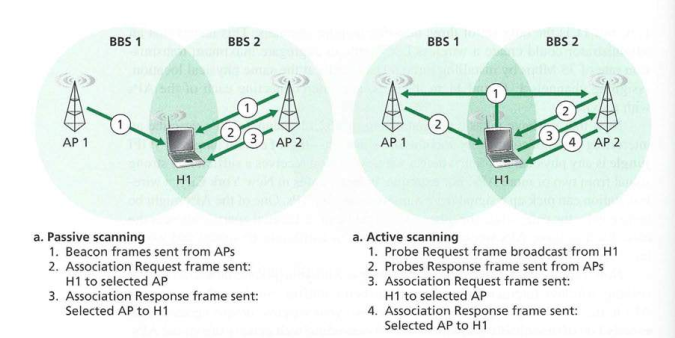
\includegraphics[width=0.8\textwidth]{img/wireless/wlan scanning.png}
      \caption{The two scanning methods}
    \end{figure}
  \end{subsection}
\end{section}
\begin{section}{Problems with 802.11}
  As already said in the chapter about wireless, the medium is unrealibale and the channel is shared, so
  there are some problems that have to be addressed.
  \begin{subsection}{Hidden terminal problem}
    The hidden terminal problem is a problem that arises when two stations can't hear each other, but they
    can hear the same access point.\\
    This can happen, for example, when two stations are too far from each other, but they are close 
    to the AP, or there's an obstacle between them.\\
    This problem is illustrated in figure \ref{fig:hidden terminal problem}.
    \begin{figure}[h]
      \centering
      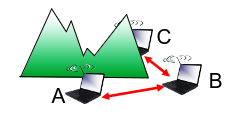
\includegraphics[width=0.5\textwidth]{img/wireless/hidden terminal problem.png}
      \caption{Hidden terminal problem}
      \label{fig:hidden terminal problem}
    \end{figure}
    Suppose that Station A is transmitting to Station B, which is also receiving from Station C.\\
    Station C can't hear Station A, so it will transmit, causing a collision at Station B.
  \end{subsection}
  \begin{subsection}{Fading}
    A second scenario that results in undetectable collisions at the receiver is fading.\\
    With fading we refer to the fact that the signal loses strength as it propagates through the medium.\\
    Figure \ref{fig:fading} shows the fading problem. A and C are placed such that their signals 
    are not strong enough to detect each other's transmissions , yet their signals are strong 
    enough to interfere with each other at station B.
    \begin{figure}[h]
      \centering
      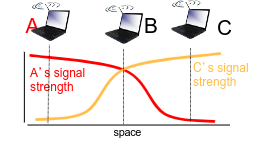
\includegraphics[width=0.5\textwidth]{img/wireless/fading.png}
      \caption{Fading}
      \label{fig:fading}
    \end{figure}
  \end{subsection}
  As previously said, 802.11 uses a half-duplex channel, so only one station can transmit at a time.
  \begin{subsection}{CSMA/CA}
    Since the channel is shared, the 802.11 standard uses CSMA/CA to avoid collisions, which is a 
    random access protocol similar to the CSMA/CD used in Ethernet.\\
    It implements collision avoidance instead of detection for two reasons:
    \begin{itemize}
      \item I requires a full duplex channel, and because the signals are very weak, it can be very
        costly to implement
      \item fading and hidden terminal problems make it difficult to detect collisions
    \end{itemize}
    For those reasons, once a station begins to transmit a frame, it transmits the frame in its 
    entirety, which, if you think about it, would increase the probability of a collision, degrading
    the performance of the network.\\
    Keep also in mind that 802.11 uses link-layer acknowledgements, so if an acknowledgement is not
    received after a certain time, it is retransmitted, and after a certain number of retransmissions,
    the frame is dropped.
    The CSMA/CA protocol is as follows: suppose that a station wants to transmit a frame
    \begin{enumerate}
      \item If initially the station senses the channel idle, it transmits its frame after a short 
        period of time known as the Distributed Inter-frame Space (DIFS)
      \item Otherwise, the station chooses a random backoff value using binary exponential backoff 
         and counts down this value after DIFS when the channel is sensed idle. While the channel 
         is sensed busy, the counter value remains frozen.
      \item When the counter reaches zero (note that this can only occur while the channel is 
        sensed idle), the station transmits the entire frame and then waits for an acknowledgment.
      \item If an acknowledgment is received, the transmitting station knows that its frame has 
        been correctly received at the destination station. If the station has another 
        frame to send, it begins the CSMA/CA protocol at step 2. If the acknowledgment isn't 
        received, the transmitting station reenters the backoff phase in step 2, with the random 
        value chosen from a larger interval.
    \end{enumerate}
    The goal is thus avoiding collisions whenever possible, hoping that by choosing a random
    backoff value, the stations will not choose the same value, and thus will not transmit at the
    same time.\\
    \begin{subsubsection}{RTS and CTS}
      802.11 also includes a optional reservation scheme, which is used to reserve the channel before
      transmitting a frame.\\
      The station that wants to transmit a frame can send a short \textbf{Request to Send(RTS)} 
      control frame and a short \textbf{Clear to Send(CTS)} control frame to \textit{reserve} the
      access to the channel.\\
      When a sender wants to send a DATA frame, it can first send an RTS frame to the AP, indicating 
      the total time required to transmit the DATA frame and the acknowledgment (ACK) frame. When 
      the AP receives the RTS frame , it responds by broadcasting a CTS frame. This CTS frame serves 
      two purposes: It gives the sender explicit permission to send and also instructs the other 
      stations not to send for the reserved duration.\\
      This technique make other station refrain from sending, thus reducing the probability of
      collisions, and solving the hidden terminal problem, at the cost of a higher overhead.\\
      \begin{figure}[h]
        \centering
        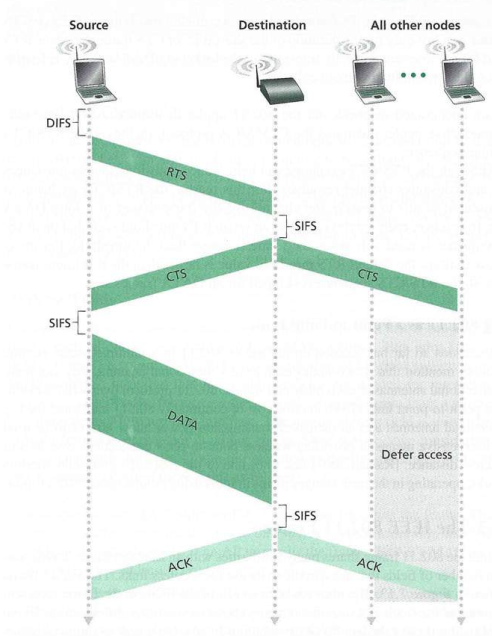
\includegraphics[width=0.5\textwidth]{img/wireless/cmsa with RTS.png}
        \caption{Collision avoidance with RTS/CTS}
      \end{figure}

    \end{subsubsection}

  \end{subsection}
\end{section}
\begin{section}{802.11 Features}
  \begin{subsection}{Frame Addressing}
    Although the 802.11 frame shares many similarities with an Ethernet frame, it also contains a 
    number of fields that are specific to its use for wireless links.\\
    The frame format is shown in figure \ref{fig:80211 frame format}.
    \begin{figure}[h]
      \centering
      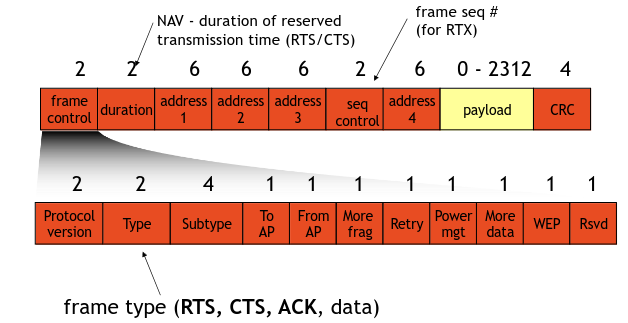
\includegraphics[width=0.5\textwidth]{img/wireless/802.11 frame.png.png}
      \caption{802.11 frame format}
      \label{fig:80211 frame format}
    \end{figure}
  \end{subsection}
  The numbers above each of the fields in the frame represent the lengths of the fields in bytes.
  The duration field is used to indicate the amount of time required to transmit the frame, and is 
  used for power saving.\\
  After that there are 4 address fields:
  \begin{itemize}
    \item The \textbf{address 1} is the MAC address of the station that is to receive the frame.
    \item The \textbf{address 2} is the MAC address of the station that is transmitting 
      the frame.
    \item The \textbf{address 3} contains the MAC address of the router interface of the subnet.
    \item The \textbf{address 4} is used in ad-hoc mode, and is the MAC address of the 
      destination station.
  \end{itemize}
  \begin{subsection}{Rate adaptation}
    802.11 also supports rate adaptation, which is the ability to change the transmission rate 
    based on the quality of the channel.\\
    This is necessary because the channel conditions can change rapidly, especially with mobile
    stations. In fact, As node moves away from base station, SNR decreases, BER(Bit Error Rate) increases
    If the modulation technique used in the 802.11 protocol operating between the base
    station and the user does not change, the BER will become unacceptably high as the
    SNR decreases, and eventually no transmitted frames will be received correctly.
    Base station and mobile dynamically change transmission rate (physical layer modulation technique) 
    as the mobile station moves, and the SNR varies as a result.
  \end{subsection}
  \begin{subsection}{Power Management}
    Power is a precious resource in mobile devices, and thus the 802.11 standard provides 
    power-management capabilities that allow 802.11 nodes to minimize the amount of time that 
    their sense, transmit, and receive functions and other circuitry need to be "on".\\
    A node is able to explicitly alternate between sleep and wake states. A node indicates to the 
    access point that it will be going to sleep by setting the power-management bit in the header 
    of an frame. A timer in the node is then set to wake up the node just before the AP is 
    scheduled to send its beacon frame.\\
    Since the AP knows from the set power-transmission bit that the node is going to sleep, it wont send any
    , and will buffer any frames destined for the sleeping host for later transmission.\\
    A node will wake up just before the AP sends a beacon frame, and quickly enter the fully active 
    state.
    The beacon frames sent out by the AP contain a list of nodes whose frames have been buffered 
    at the AP. If there are no buffered frames for the node, it can go back to sleep. Otherwise, 
    the node can explicitly request that the buffered frames be sent by sending a polling message 
    to the AP.

    \begin{figure}[h]
      \centering
      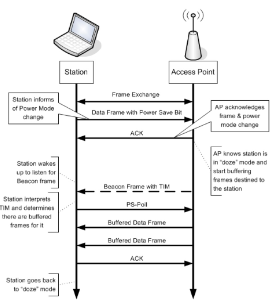
\includegraphics[width=0.5\textwidth]{img/wireless/80211 power saving.png}
      \caption{Power management in 802.11}
    \end{figure}

  \end{subsection}

\end{section}


